\subsection{Forward pass in convolution layer}
\begin{align*}
Z^{\text{conv}}[:,:,k] &= \sum_{c=1}^{C_{in}} W[:,:,c,k] * X[:,:,c] \\
Z[:,:,k] &= Z^{\text{conv}} + b[k] \\
A[:,:,k] &= \sigma(Z[:,:,k])
\end{align*}

\subsection{Adam optimization}
\textbf{Adam} (Adaptive Moment Estimation) is a widely used optimization algorithm in training neural networks. It combines the advantages of \textbf{AdaGrad} (adaptive learning rates for individual parameters) and \textbf{RMSprop} (using a moving average of squared gradients). Adam is effective due to its ability to adaptively adjust the learning rate for each parameter based on estimates of the first-order moments (mean) and second-order moments (variance) of the gradients.

\subsection*{Basic Steps:}
Given a learning rate $\alpha$, decay rates $\beta_1, \beta_2 \in [0, 1)$, and a small constant $\epsilon$ to prevent division by zero.
\begin{enumerate}
    \item Initialize moment vectors: $m_0 = \mathbf{0}$, $v_0 = \mathbf{0}$.
    \item For each iteration $t = 1, 2, \dots$:
    \begin{itemize}
        \item Compute the gradient $g_t$ of the loss function at time $t$:
        $$g_t = \nabla_\theta J(\theta_{t-1})$$
        \item Update biased first moment estimate (mean of gradients):
        $$m_t = \beta_1 m_{t-1} + (1 - \beta_1) g_t$$
        \item Update biased second moment estimate (mean of squared gradients):
        $$v_t = \beta_2 v_{t-1} + (1 - \beta_2) g_t^2$$
        \item Perform bias correction for the moments (to counteract initial values being zero):
        $$\hat{m}_t = \frac{m_t}{1 - \beta_1^t}$$
        $$\hat{v}_t = \frac{v_t}{1 - \beta_2^t}$$
        \item Update model parameters:
        $$\theta_t = \theta_{t-1} - \alpha \frac{\hat{m}_t}{\sqrt{\hat{v}_t} + \epsilon}$$
    \end{itemize}
\end{enumerate}

\subsection*{Advantages:}
\begin{itemize}
    \item \textbf{Efficiency:} Performs well in practice across various machine learning tasks.
    \item \textbf{Adaptive:} Adjusts the learning rate for each parameter, leading to faster convergence.
    \item \textbf{Ease of Use:} Does not require extensive hyperparameter tuning; default values often yield good results.
\end{itemize}

\subsection{Regularization}
\begin{itemize}
    \item L2 regularization (weight decay) and dropout help prevent overfitting.
    \item Dropout encourages robust feature learning.
\end{itemize}

\subsection{Other Techniques}
\begin{itemize}
    \item \textbf{Data augmentation}: enhances generalization.
    \item \textbf{Global average pooling}: reduces parameters.
\end{itemize}

\subsection{Example models in the book}
\begin{figure}[!h]
    \centering
    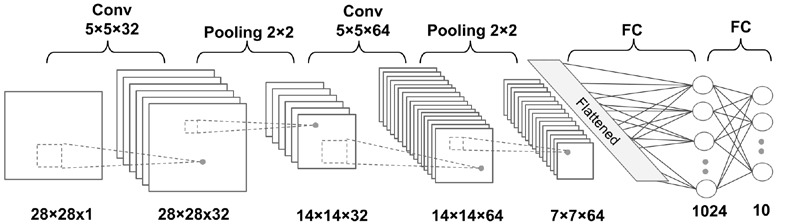
\includegraphics[width=0.9\textwidth]{../figures/deepCNN.jpg}
    \caption{A deep CNN}
\end{figure}
